\documentclass{article}

\usepackage{geometry}
\usepackage{xeCJK}
\usepackage{amsmath}
\usepackage{bm}
\usepackage{tikz}
\usepackage{pgfplots}
\usepackage{pst-func}
% figure[H] float
\usepackage{float}
% subfigure
\usepackage{subcaption}
\usepackage{amssymb}
\usepackage{hyperref}
\usepackage{setspace}
% 字体底部样式:下划线、波浪线等
\usepackage{ulem}
% 修改公式编号
\usepackage{chngcntr}
% 提供修改列表的编号样式的功能
\usepackage{enumitem}
% 提供对角线的省略号
\usepackage{mathdots}
\usepackage{arydshln}

% make cdot thicker,比 cdot 更粗的圆点
\makeatletter
\newcommand*\bigcdot{\mathpalette\bigcdot@{.5}}
\newcommand*\bigcdot@[2]{\mathbin{\vcenter{\hbox{\scalebox{#2}{$\m@th#1\bullet$}}}}}
\makeatother

% 设置行间距 1.5 倍
\renewcommand{\baselinestretch}{1.5}
% 自定义图片的标题:Figure -> 图
\renewcommand{\figurename}{图}
% 自定义表格的标题:Table -> 表
\renewcommand{\tablename}{表}
% 字符外添加圆圈
\newcommand*\circled[1]{
\tikz[baseline=(char.base)]{
   \node[shape=circle,draw,inner sep=1pt] (char) {#1};
}}

% 设置页大小和页边距,或者scale=0.8
\geometry{a4paper,left=3.18cm,right=3.18cm,top=2.54cm,bottom=2.54cm}
% 兼容
\pgfplotsset{compat=1.16}
% 中文默认没有斜体和粗体格式,开启伪斜体和指定黑体;
\setCJKmainfont[AutoFakeSlant, BoldFont=SimHei]{SimSun}

\hypersetup{
    colorlinks,
    citecolor=black,
    filecolor=black,
    linkcolor=black,
    urlcolor=black
}
% 每个章节后,重置公式编号
\counterwithin*{equation}{section}

% 修改公式标签引用颜色
\def\eqref#1{{\color{blue}\hypersetup{linkcolor=blue} (\ref{#1}) }}
% 修改图片标签引用的颜色
\def\figureref#1{{\color{blue}\hypersetup{linkcolor=blue} (\ref{#1}) }}
% 修改跳转标签引用的颜色
\def\linkref[#1]#2{\hyperref[#1]{\color{blue}\ #2\ }}
% 引用 section 的章节号
\def\secref#1{\hyperref[#1]{\color{blue}[\ref{#1}节]}}

% 缩进
\usepackage{indentfirst}
\makeatletter
\def\paragraph{
    \parindent2em
}
\makeatother

\begin{document}
  \tableofcontents

  \newpage
  \section{行列式}
    \subsection{二阶行列式}
\subsubsection{二元线性方程组}
\paragraph{}
用消元法解二元线性方程组
\begin{align}
\label{消元法解二元线性方程组}
\begin{split}
  \left\{ \begin{array}{l}
    a_{11}x_1 + a_{12}x_2 = b_1, \\
    a_{21}x_1 + a_{22}x_2 = b_2.
  \end{array} \right.
\end{split}
\end{align}

\paragraph{}
为消去未知数$x_2$,以$a_{22}$与$a_{12}$分别乘上列两方程的两端,然后两个方程相减,得
\begin{equation*}
  (a_{11}a_{22} - a_{12}a_{21})x_1 = b_1a_{22} - a_{12}b_2;
\end{equation*}
类似地,消去$x_1$,得
\begin{equation*}
  (a_{11}a_{22} - a_{12}a_{21})x_2 = a_{11}b_2 - b_1a_{21}.
\end{equation*}

\paragraph{}
当$a_{11}a_{22} - a_{12}a_{21} \neq 0$时,求得方程组\eqref{消元法解二元线性方程组}的解为
\begin{equation}
  \label{二元线性方程组的解}
  x_1 = \frac{ b_1a_{22} - a_{12}b_2 }{ a_{11}a_{22} - a_{12}a_{21} }, \; x_2 = \frac{ a_{11}b_2 - b_1a_{21} }{ a_{11}a_{22} - a_{12}a_{21} }.
\end{equation}

\subsubsection{二阶行列式}
\paragraph{}
其中分母$a_{11}a_{22} - a_{12}a_{21}$ 是由方程组\eqref{消元法解二元线性方程组}的四个系数确定的,把这四个数按它们在方程组\eqref{消元法解二元线性方程组}中的位置,排成二行二列的数表
\begin{equation}
\label{二阶数表}
\begin{array}{ll}
a_{11} & a_{12} \\ a_{21} & a_{22},
\end{array}
\end{equation}
表达式$a_{11}a_{22} - a_{12}a_{21}$称为数表\eqref{二阶数表}所确定的\textbf{二阶行列式},并记作
\begin{equation}
  \left|
  \begin{array}{ll}
  a_{11} & a_{12} \\ a_{21} & a_{22}
  \end{array} \right|.
\end{equation}

\subsubsection{对角线法则}
\paragraph{}
二阶行列式的定义,可以用\textbf{对角线法则}来记忆。$a_{11}$到$a_{22}$的实线称为\textbf{主对角线},$a_{12}$到$a_{21}$的虚线称为\textbf{副对角线}。于是二阶行列式便是:主对角线上的两元素之积减去副对角线上的两元素之积所得的差。
\begin{figure}[H]
\centering
  % 二阶行列式的对角线法则
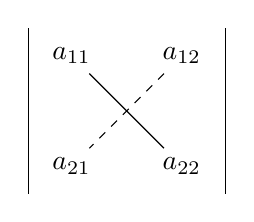
\begin{tikzpicture}
  \draw (-1.25,1.05) -- (-1.25,-1.05);

  \node at (-.7,.7) (a11) {$a_{11}$};
  \node at (.7,-.7) (a22) {$a_{22}$};
  \draw (a11) -- (a22);

  \node at (.7,.7) (a12) {$a_{12}$};
  \node at (-.7,-.7) (a21) {$a_{21}$};
  \draw[dashed] (a12) -- (a21);

  \draw (1.25,1.05) -- (1.25,-1.05);
\end{tikzpicture}

  \caption{对角线法则}
  \label{图:二阶对角线法则}
\end{figure}

\subsubsection{二元线性方程组的解}
\paragraph{}
利用二阶行列式的概念和对角线法则,\eqref{二元线性方程组的解}式中$x_1,x_2$的分子也可写成二阶行列式,即
\begin{equation*}
  b_1a_{22} - a_{12}b_2 = \left|\begin{array}{ll} b_1 & a_{12} \\ b_2 & a_{22}\end{array}\right|, \;
  a_{11}b_2 - b_1a_{21} = \left|\begin{array}{ll} a_{11} & b_1 \\ a_{21} & b_2\end{array}\right|,
\end{equation*}

\paragraph{}
若记
\begin{equation*}
  D = \left|\begin{array}{ll} a_{11} & a_{12} \\ a_{21} & a_{22} \end{array}\right|, \;
  D_1 = \left|\begin{array}{ll} b_1 & a_{12} \\ b_2 & a_{22} \end{array}\right|, \;
  D_2 = \left|\begin{array}{ll} a_{11} & b_1 \\ a_{21} & b_2 \end{array}\right|, \;
\end{equation*}
那么\eqref{二元线性方程组的解}式可写成
\begin{equation*}
  x_1 = \frac{D_1}{D} = \frac{\left|\begin{array}{ll} b_1 & a_{12} \\ b_2 & a_{22} \end{array}\right|}{\left|\begin{array}{ll} a_{11} & a_{12} \\ a_{21} & a_{22} \end{array}\right|}, \;
  x_2 = \frac{D_2}{D} = \frac{\left|\begin{array}{ll} a_{11} & b_1 \\ a_{21} & b_2 \end{array}\right|}{\left|\begin{array}{ll} a_{11} & a_{12} \\ a_{21} & a_{22} \end{array}\right|}.
\end{equation*}

\paragraph{}
注意,这里的分母$D$是由方程组\eqref{消元法解二元线性方程组}的系数所确定的二阶行列式(称系数行列式),$x_1$的分子$D_1$是常数项$b_1,b_2$替换$D$中$x_1$的系数$a_{11}, a_{21}$(第$1$列)所得的二阶行列式;$x_2$的分子$D_2$是用常数项$b_1, b_2$替换$D$中$x_2$的系数$a_{12}, a_{22}$(第$2$列)所得的二阶行列式。

\subsection{三阶行列式}
\subsubsection{定义}
\paragraph{}
\textbf{定义~~}设有$9$个数排成$3$行$3$列的数表
\begin{equation}
  \label{三阶数表}
  \begin{array}{lll}
    a_{11} & a_{12} & a_{13} \\
    a_{21} & a_{22} & a_{23} \\
    a_{31} & a_{32} & a_{33},
  \end{array}
\end{equation}
记
\begin{align}
\centering
  \begin{split}
    \label{三阶行列式}
    &\;\left|\begin{array}{lll}
      a_{11} & a_{12} & a_{13} \\
      a_{21} & a_{22} & a_{23} \\
      a_{31} & a_{32} & a_{33}
    \end{array}\right| \\
    =&\; a_{11}a_{22}a_{33} + a_{12}a_{23}a_{31} + a_{13}a_{21}a_{32} - \\
    &\; a_{11}a_{23}a_{32} - a_{12}a_{21}a_{33} - a_{13}a_{22}a_{31},
  \end{split}
\end{align}
\eqref{三阶行列式}称为数表\eqref{三阶数表}所确定的三阶行列式。

\subsubsection{对角线法则}
\begin{figure}[H]
\centering
  % 三阶行列式的对角线法则
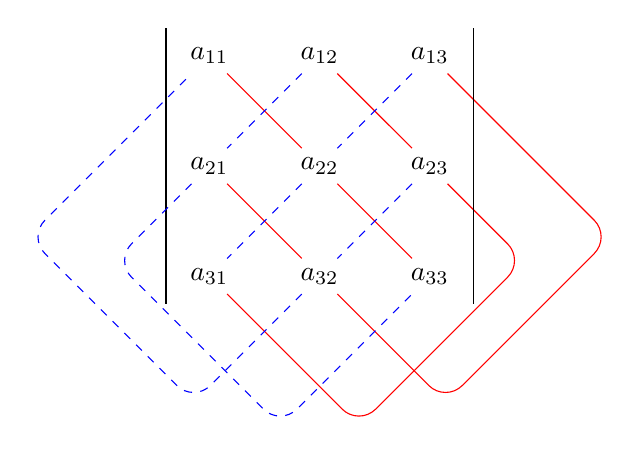
\begin{tikzpicture}

  \draw (-1.95,1.75) -- (-1.95,-1.75);

  \node at (-1.4,1.4) (a11) {$a_{11}$};
  \node at (0,1.4) (a12) {$a_{12}$};
  \node at (1.4,1.4) (a13) {$a_{13}$};

  \node at (-1.4,0) (a21) {$a_{21}$};
  \node at (0,0) (a22) {$a_{22}$};
  \node at (1.4,0) (a23) {$a_{23}$};

  \node at (-1.4,-1.4) (a31) {$a_{31}$};
  \node at (0,-1.4) (a32) {$a_{32}$};
  \node at (1.4,-1.4) (a33) {$a_{33}$};

  \draw[red] (a11) -- (a22) -- (a33);
  \draw[red,rounded corners=3mm] (a12) -- (a23) -- (2.6,-1.2) -- (0.5,-3.3) -- (a31);
  \draw[red,rounded corners=3mm] (a21) -- (a32) -- (1.6,-3) -- (3.7,-0.9) -- (a13);

  \draw[dashed,blue] (a13) -- (a22) -- (a31);
  \draw[dashed,blue,rounded corners=3mm] (a12) -- (a21) -- (-2.6,-1.2) -- (-0.5,-3.3) -- (a33);
  \draw[dashed,blue,rounded corners=3mm] (a23) -- (a32) -- (-1.6,-3) -- (-3.7,-0.9) -- (a11);

  \draw (1.95,1.75) -- (1.95,-1.75);
\end{tikzpicture}

  \caption{对角线法则}
  \label{图:三阶对角线法则}
\end{figure}

\paragraph{}
对角线法则只适用于二阶与三阶行列式,下面先介绍全排列及其逆序数,然后由此引出$n$阶行列式的概念。

\subsection{全排列及其逆序数}
\subsubsection{全排列}
\paragraph{}
把$n$个不同的元素排成一列,叫做这$n$个元素的\textbf{全排列}(简称\textbf{排列})。

\paragraph{}
从$n$个元素中任取一个放在第一个位置上,有$n$种取法;又从剩下的$n-1$个元素中任取一个放在第二个位置上,有$n-1$种取法;依此类推,于是:
\begin{equation*}
  P_n = n \bigcdot (n-1) \bigcdot \cdots \bigcdot 3 \bigcdot 2 \bigcdot 1 = n!.
\end{equation*}

\subsubsection{逆序数}
\paragraph{}
概念:
\begin{enumerate}
  \item \textbf{标准次序}:$n$个不同的自然数,按由小到大的顺序排序
  \item \textbf{逆序}:当某两个元素的先后次序与标准次序不同时,就说有$1$个\uwave{逆序}
  \item \textbf{排列的逆序数}:一个排列中所有逆序的总数
  \item \textbf{奇/偶排列}:逆序数为奇/偶数
\end{enumerate}

\paragraph{}
下面讨论计算排列的逆序数的方法:

\paragraph{}
一般性,设$n$个元素为$1$至$n$这$n$个自然数,并规定由小到大为标准次序,设:
\begin{equation*}
  p_1p_2\cdots p_n
\end{equation*}
为这$n$个自然数的一个排列,考虑元素$p_i(i=1,2,\cdots,n)$,如果比$p_i$大的且排在$p_i$前面的元素有$t_i$个,就说$p_i$这个元素的逆序数是$t_i$。全体元素的逆序数之总和
\begin{equation*}
  t = t_1 + t_2 + \cdots + t_n = \sum_{t=1}^n t_i,
\end{equation*}
即是这个排列的逆序数。

\subsection{$n$阶行列式的定义}

\subsection{对换}

\subsection{行列式的性质}

\subsection{行列式按行(列)展开}

\subsection{克拉默法则}

  \section{矩阵及其运算}
    \subsection{矩阵的概念}
\subsubsection{概念}
\paragraph{}
\textbf{定义~~}由$m\times n$个数$a_{ij} (i=1,2,\cdots,m; \; j =1,2,\cdots,n)$排成的$m$行$n$列的数表
\begin{equation*}
  \left|\begin{array}{cccc}
    a_{11} & a_{12} & \cdots & a_{1n} \\
    a_{21} & a_{22} & \cdots & a_{2n} \\
    \vdots & \vdots &  & \vdots \\
    a_{m1} & a_{m2} & \cdots & a_{mn}
  \end{array} \right|
\end{equation*}
称为\textbf{$m$行$n$列矩阵},简称\textbf{$m \times n$ 矩阵},记作
\begin{equation}
  A = \left[\begin{array}{cccc}
  a_{11} & a_{12} & \cdots & a_{1n} \\
  a_{21} & a_{22} & \cdots & a_{2n} \\
  \vdots & \vdots &  & \vdots \\
  a_{m1} & a_{m2} & \cdots & a_{mn}
\end{array} \right]
\end{equation}
也记作$A_{m\times n}$

\paragraph{}
行数和列数都等于$n$的矩阵称为\textbf{$n$阶矩阵}或\textbf{$n$阶方阵}。$n$阶矩阵$A$也记作$A_n$。

\paragraph{}
只有一行的矩阵
\begin{equation*}
  A = (a_1a_2\cdots a_n)
\end{equation*}
称为\textbf{行矩阵},又称\textbf{行向量}。为了避免元素间的混淆,也记作
\begin{equation*}
  A = (a_1,a_2,\cdots,a_n).
\end{equation*}

\paragraph{}
只有一列的矩阵
\begin{equation*}
  B = \left[\begin{array}{c}
    b_1 \\
    b_2 \\
    \cdots \\
    b_m
  \end{array}\right]
\end{equation*}
称为\textbf{列矩阵},又称\textbf{列向量}。

\paragraph{}
两个矩阵的行数相等、列数也相等时,就称它们是\textbf{同型矩阵}。如果$A=(a_{ij})$与$B=(b_{ij})$是同型矩阵,并且它们的对应元素相等,即
\begin{equation*}
  a_{ij}=b_{ij} \;(i=1,2,\cdots,m; \; j=1,2,\cdots,n),
\end{equation*}
那么就称矩阵$A$与矩阵$B$\textbf{相等},记作
\begin{equation*}
  A=B.
\end{equation*}

\subsubsection{类型}
\paragraph{}
元素都是零的矩阵称为\textbf{零矩阵},记作$O$。注意不同型的零矩阵是不同的。

\paragraph{}
主对角线上的元素都是$1$,其余都为$0$的$n$阶矩阵,叫做$n$阶\textbf{单位矩阵},记作$E$
\begin{equation*}
  E = \left[\begin{array}{cccc}
    1 & 0 & \cdots & 0 \\
    0 & 1 & \cdots & 0 \\
    \vdots & \vdots & & \vdots \\
    0 & 0 & \cdots & 1
  \end{array}\right]
\end{equation*}

\paragraph{}
不在主对角线上的元素都是$0$,称为\textbf{对角矩阵},记作$A = diag(\lambda_1,\lambda_2,\cdots,\lambda_n)$
\begin{equation*}
  A = \left[\begin{array}{cccc}
    \lambda_1 & 0 & \cdots & 0 \\
    0 & \lambda_2 & \cdots & 0 \\
    \vdots & \vdots & & \vdots \\
    0 & 0 & \cdots & \lambda_n
  \end{array}\right]
\end{equation*}

\paragraph{}
\textbf{由于矩阵和线性变换之间存在一一对应的关系,因此可以利用矩阵来研究线性变换,也可以利用线性变换来解析矩阵的含义。}

\subsection{矩阵的运算}
\paragraph{}

\subsection{逆矩阵}
\paragraph{}

\subsection{矩阵的分块法}
\paragraph{}

  \section{矩阵的初等变换与线性方程组}
    \paragraph{}
\begin{enumerate}
  \item 引入矩阵的初等变换,建立矩阵的秩的概念,以及秩的性质。
  \item 利用矩阵的秩,讨论线性方程组无解、有唯一解或有无穷多解的充分必要条件。
  \item 介绍用初等变换解线性方程组的方法。
\end{enumerate}

\subsection{矩阵的初等变换}
\subsubsection{初等变换的引例}
\paragraph{}
消元法解线性方程组例子

\paragraph{}
\textbf{引例~~}求解线性方程组
\begin{equation*}
  \left\{\begin{array}{c}
            2x_1 - \enspace x_2 - \enspace x_3 + \enspace x_4 = 2, \; \circled{1} \\
    \enspace x_1 + \enspace x_2 -         2x_3 + \enspace x_4 = 4, \; \circled{2} \\
            4x_1 -         6x_2 +         2x_3 -         2x_4 = 4, \; \circled{3} \\
            3x_1 +         6x_2 -         9x_3 +         7x_4 = 9, \; \circled{4}
  \end{array} \right. \tag{$A$}
\end{equation*}

\paragraph{}
\textbf{解~~}
\begin{alignat*}{3}
  (A)\, & \xrightarrow[\circled{\tiny 3} \,\div\, 2]{\circled{\tiny 1} \,\leftrightarrow\, \circled{\tiny 2}} & \;
  \left\{\begin{array}{ll}
    \enspace x_1 + \enspace x_2 -         2x_3 + \enspace x_4 = 4, & \circled{1} \\
            2x_1 - \enspace x_2 - \enspace x_3 + \enspace x_4 = 2, & \circled{2} \\
            2x_1 -         3x_2 + \enspace x_3 - \enspace x_4 = 2, & \circled{3} \\
            3x_1 +         6x_2 -         9x_3 +         7x_4 = 9, & \circled{4}
  \end{array} \right. \tag{$A_1$} \\
  % ----------------------------------------------------------------------------
  & \xrightarrow[\circled{\tiny 4} \,-\, 3\circled{\tiny 1}]{\substack{\circled{\tiny 2} \,-\, \circled{\tiny 3} \\ \circled{\tiny 3} \,-\, 2\circled{\tiny 1}}} & \;
  \left\{\begin{array}{rl}
     x_1 + x_2 - 2x_3 + \enspace x_4 = \hspace{0.8em} 4, & \circled{1} \\
          2x_2 - 2x_3 +         2x_4 = \hspace{0.8em} 0, & \circled{2} \\
         -5x_2 + 5x_3 -         3x_4 =               -6, & \circled{3} \\
          3x_2 - 3x_3 +         4x_4 =               -3, & \circled{4}
  \end{array} \right. \tag{$A_2$} \\
  % ----------------------------------------------------------------------------
  & \xrightarrow[\substack{\circled{\tiny 3} \,+\, 5\circled{\tiny 2} \\ \circled{\tiny 4} \,-\, 3\circled{\tiny 2}}]{\circled{\tiny 2} \,\times\, \frac{1}{2}} & \;
  \left\{\begin{array}{rl}
     x_1 + x_2 -         2x_3 + \enspace x_4 = \hspace{0.8em} 4, & \circled{1} \\
           x_2 - \enspace x_3 + \enspace x_4 = \hspace{0.8em} 0, & \circled{2} \\
                                        2x_4 = -6, & \circled{3} \\
                                         x_4 = -3, & \circled{4}
  \end{array} \right. \tag{$A_3$} \\
  % ----------------------------------------------------------------------------
  & \xrightarrow[\circled{\tiny 4} \,-\, 2\circled{\tiny 3}]{\circled{\tiny 3} \,\leftrightarrow\, \circled{\tiny 4}} & \;
  \left\{\begin{array}{rrrl}
     x_1 + & x_2 - 2x_3 + & x_4 = \hspace{0.8em} 4, & \circled{1} \\\cdashline{1-1}[1pt/1pt]
     \multicolumn{1}{l;{1pt/1pt}}{} & x_2 - \enspace x_3 + & x_4 = \hspace{0.8em} 0, & \circled{2} \\\cdashline{2-2}[1pt/1pt]
     \multicolumn{2}{l;{1pt/1pt}}{} & x_4 = -3, & \circled{3} \\\cdashline{3-4}[1pt/1pt]
     & & 0 = \hspace{0.8em} 0, & \circled{4}
  \end{array} \right. \tag{$A_4$}
\end{alignat*}

\subsubsection{初等变换的定义}
\paragraph{}
\textbf{定义~~}下面三种变换称为矩阵的\textbf{初等行变换}:
\begin{enumerate}
  \item 对调两行(对调$i,j$两行,记作$r_i \leftrightarrow r_j$);
  \item 以数$k \neq 0$乘某一行中的所有元素(第$i$行乘$k$,记作$r_i \times k$);
  \item 把某一行所有元素的$k$倍加到另一行对应的元素上去(第$j$行的$k$倍,加到第$i$行上,记作$r_i + kr_j$)。
\end{enumerate}
相同地,可得到\textbf{初等列变换}的定义。

\paragraph{}
矩阵$A$经过有限次初等变换变成矩阵$B$,就称\textbf{矩阵$A$与$B$等价},记作$A\sim B$。仅有行/列变换,可记作$A\overset{r}{\sim}B$或$A\overset{c}{\sim}B$

\paragraph{}
矩阵之间的等价关系具有下列性质:
\begin{enumerate}
  \item \textbf{反身性~~$A\sim A$};
  \item \textbf{对称性~~若$A\sim B$,则$B\sim A$};
  \item \textbf{传递性~~若$A\sim B, B\sim C$,则$A\sim C$}。
\end{enumerate}

\subsubsection{行阶梯形矩阵}
\paragraph{}
\textbf{行阶梯形矩阵~~}可画出一条阶梯线,线的下方全为$0$,每个台阶只有一行,台阶数即是非零行的行数。阶梯线的竖线后面的第一个元素为非零元。例如,
\begin{equation*}
\left[\begin{array}{rrrrr}
  {\color{red!50}1} & 1 & -2 & 1 & 4 \\\cdashline{1-1}[1pt/1pt]
  \multicolumn{1}{r;{1pt/1pt}}{{\color{gray!50}0}} & {\color{red!50}1} & -1 & 1 & 0 \\\cdashline{2-3}[1pt/1pt]
  {\color{gray!50}0} & {\color{gray!50}0} & \multicolumn{1}{r;{1pt/1pt}}{{\color{gray!50}0}} & {\color{red!50}1} & -3 \\\cdashline{4-5}[1pt/1pt]
  {\color{gray!50}0} & {\color{gray!50}0} & {\color{gray!50}0} & 0 & {\color{gray!50}0}
\end{array}\right]
\end{equation*}

\paragraph{}
\textbf{行最简形矩阵~~}非零行的第一个非零元为$1$,且这些非零元所在的列的其它元素都为$0$。例如,
\begin{equation*}
  \left[\begin{array}{rrrrr}
    {\color{red!50}1} & {\color{blue!50}0} & -1 & {\color{blue!50}0} & 4 \\\cdashline{1-1}[1pt/1pt]
    \multicolumn{1}{r;{1pt/1pt}}{{\color{gray!50}0}} & {\color{red!50}1} & -1 & {\color{blue!50}0} & 3 \\\cdashline{2-3}[1pt/1pt]
    {\color{gray!50}0} & {\color{gray!50}0} & \multicolumn{1}{r;{1pt/1pt}}{{\color{gray!50}0}} & {\color{red!50}1} & -3 \\\cdashline{4-5}[1pt/1pt]
    {\color{gray!50}0} & {\color{gray!50}0} & {\color{gray!50}0} & {\color{gray!50}0} & {\color{gray!50}0}
  \end{array}\right]
\end{equation*}

\paragraph{}
对于任何矩阵$A_{m\times n}$,总可经过有限次初等行变换把它变为行阶梯形矩阵和行最简形矩阵(归纳法可证)。

\paragraph{}
\textbf{标准形~~}矩阵的左上角是一个单位矩阵,其余元素全为$0$。例如,
\begin{equation*}
  \left[{\color{gray!50} \begin{array}{ccccc}
    {\color{red!50}1} & 0 & 0 & 0 & 0 \\
    0 & {\color{red!50}1} & 0 & 0 & 0 \\
    0 & 0 & {\color{red!50}1} & 0 & 0 \\
    0 & 0 & 0 & 0 & 0
  \end{array}}\right]
\end{equation*}

\paragraph{}
对于$m\times n$矩阵$A$,总可经过初等变换把它化为标准形
\begin{equation*}
  F = \left[\begin{array}{cc}
    E_r & O \\
    O & O
  \end{array}\right]_{m\times n}
\end{equation*}

\subsubsection{初等变换的性质}\label{sec:初等变换的性质}
\paragraph{}
\textbf{定理1~~}设$A$与$B$为$m\times n$矩阵,那么:
\begin{enumerate}
  \item $A \overset{r}{\sim} B$的充分必要条件是存在$m$阶可逆矩阵$P$,使$PA = B$;
  \item $A \overset{c}{\sim} B$的充分必要条件是存在$n$阶可逆矩阵$Q$,使$AQ = B$;
  \item $A \sim B$的充分必要条件是存在$m$阶可逆矩阵$P$,以及$n$阶可逆矩阵$Q$,使$PAQ = B$。
\end{enumerate}

\paragraph{}
证明参考\secref{sec:定理1的证明}

\subsubsection{初等矩阵的定义}
\paragraph{}
由单位阵$E$经过一次初等变换得到的矩阵称为\textbf{初等矩阵}。
\begin{enumerate}
  \item 单位阵中第$i,j$两行对调(或第$i,j$两列对调),得初等矩阵
  \begin{equation*}
    E(i,j) = \left[\begin{array}{ccccccccccc}
      1 & & & & & & & & & & \\
        & \ddots & & & & & & & & & \\
        &        & 1 & & & & & & & & \\
        &        &   & 0 & & \cdots & &  1 & & & \\
        &        &   &   & 1 & & & & & & \\
        &        &   & \vdots  &   & \ddots & & \vdots & & & \\
        &        &   &   &   &        & 1 & & & & \\
        &        &   & 1 &   &    \cdots    &  & 0 &  & & \\
        &        &   &   &   &        &   &   & 1 &  & \\
        &        &   &   &   &        &   &   &   & \ddots & \\
        &        &   &   &   &        &   &   &   &        & 1
    \end{array}\right]\begin{array}{c}
      \\
      \\
      \\
      \leftarrow\text{第$i$行} \\
      \\
      \\
      \\
      \leftarrow\text{第$j$行} \\
      \\
      \\
      \\
    \end{array}
  \end{equation*}
  矩阵$A$的第$i,j$行交换,相当于用$m$阶初等矩阵$E_m(i,j)$左乘矩阵$A_{m\times n}$。\\
  矩阵$A$的第$i,j$列交换,相当于用$n$阶初等矩阵$E_n(i,j)$右乘矩阵$A_{m\times n}$。
  \item 以数$k\neq 0$乘单位阵的第$i$行(或第$i$)列,得初等矩阵
  \begin{equation*}
    E(i(k)) = \left[\begin{array}{ccccccc}
      1 & & & & & & \\
        & \ddots & & & & & \\
        &        & 1 & & & & \\
        &        &   & k & & & \\
        &        &   &   & 1 & & \\
        &        &   &   &   & \ddots & \\
        &        &   &   &   &        & 1 \\
    \end{array}\right]\begin{array}{c}
        \\
        \\
        \\
        \leftarrow\text{第$i$行}\\
        \\
        \\
        \\
    \end{array}
  \end{equation*}
  矩阵$A$的第$i$行乘以$k$倍,相当于用$m$阶初等矩阵$E_m(i(k))$左乘矩阵$A_{m\times n}$。\\
  矩阵$A$的第$i$列乘以$k$倍,相当于用$n$阶初等矩阵$E_n(i(k))$右乘矩阵$A_{m\times n}$。
  \item 以$k$乘$E$的第$j$行加到第$i$行上,或者对列进行类似操作,得初等矩阵
  \begin{equation*}
    E(i+j(k)) = \left[\begin{array}{ccccccc}
      1 & & & & & & \\
        & \ddots & & & & & \\
        &        & 1 & \cdots & k & & \\
        &        &   & \ddots & \vdots  & & \\
        &        &   &        & 1 & & \\
        &        &   &        &   & \ddots & \\
        &        &   &        &   &        & 1 \\
    \end{array}\right]\begin{array}{c}
      \\
      \\
      \leftarrow\text{第$i$行}\\
      \\
      \leftarrow\text{第$j$行}\\
      \\
      \\
    \end{array}
  \end{equation*}
  以$E_m(i+j(k))$左乘矩阵$A$,相当于把$A$的第$j$行乘$k$加到第$i$行上。相同地,列也具有类似性质。
\end{enumerate}

\paragraph{}
归纳以上的讨论,可得

\paragraph{}
\textbf{性质1~~}设$A$是一个$m\times n$矩阵,对$A$施行一次初等行变换,相当于在$A$的左边乘以相应的$m$阶初等矩阵;对$A$施行一次初等列变换,相当于在$A$的右边乘以相应的$n$阶初等矩阵。

\paragraph{}
\textbf{性质2~~}方阵$A$可逆的充分必要条件是存在有限个初等矩阵$P_1,P_2,\cdots,P_l$,使$A = P_1P_2\cdots P_l$。

\subsubsection{定理$1$的证明}\label{sec:定理1的证明}
\paragraph{}
\secref{sec:初等变换的性质}的证明:

\paragraph{}
$(1.)$依据$A\overset{r}{\sim}B$的定义和初等矩阵的性质,有
\begin{align*}
  A \overset{r}{\sim}B \Leftrightarrow &\; A\text{经有限次初等行变换变成}B \\
  \Leftrightarrow &\;\text{存在有限个$m$阶初等矩阵}P_1,P_2,\cdots,P_l\text{,使}P_l\cdots P_2P_1A = B \\
  \Leftrightarrow &\;\text{存在$m$阶可逆矩阵$P$,使}PA=B.
\end{align*}
类似可证明$(2.)$和$(3.)$。

\paragraph{}
\textbf{推论~~}方阵$A$可逆的充分必要条件是$A\overset{r}{\sim}E$。

\subsection{矩阵的秩}
\subsubsection{定义}
\paragraph{}
给定一个$m\times n$矩阵$A$,它的标准形
\begin{equation*}
  F = \left[\begin{array}{cc}
    E_r & O \\
    O & O
  \end{array}\right]_{m\times n}
\end{equation*}
由数$r$完全确定。这个数也是$A$的行阶梯形中非零行的行数,这个数便是矩阵$A$的\textbf{秩}。

\paragraph{}
\textbf{定义1~~}在$m\times n$矩阵$A$中,任取$k$行与$k$列$(k \leq m, k \leq n)$,位于这些行列交叉处的$k^2$个元素,不改变它们在$A$中所处的位置次序,而得的$k$阶行列式,称为\textbf{矩阵$A$的$k$阶子式}。

\paragraph{}
$m\times n$矩阵$A$的$k$阶子式共有$C_m^k\bigcdot C_n^k$个。

\paragraph{}
\textbf{定义2~~}设在矩阵$A$中有一个不等于$0$的$r$阶子式$D$,且所有$r+1$阶子式(如果存在)全等于$0$,那么$D$称为矩阵$A$的\textbf{最高阶非零子式},数$r$称为\textbf{矩阵$A$的秩},记作$R(A)$。并规定零矩阵的秩等于$0$。

\paragraph{}
由于行列式与其转置行列式相等,因此$A^T$的子式与$A$的子式对应相等,从而$R(A^T)=R(A)$。

\paragraph{}
对于$n$阶矩阵$A$,由于$A$的$n$阶子式只有一个$|A|$,故当$|A|\neq 0$时$R(A)=n$,当$|A|=0$时$R(A)<n$。可见可逆矩阵的秩等于矩阵的阶数,不可逆矩阵的秩小于矩阵的阶数。因此可逆矩阵又称\textbf{满秩矩阵},不可逆矩阵(奇异矩阵)又称\textbf{降秩矩阵}。

\subsubsection{定理}
\paragraph{}
\textbf{定理~~}若$A\sim B$,则$R(A)=R(B)$。

\paragraph{}
由于$A\sim B$的充分必要条件是有可逆矩阵$P, Q$,使$PAQ=B$,因此可得

\paragraph{}
\textbf{推论~~}若可逆矩阵$P,Q$使$PAQ=B$,则$R(A)=R(B)$。

\paragraph{}
根据定理,为求矩阵的秩,只要把矩阵用初等行变换变成行阶梯形矩阵,行阶梯形矩阵中非零行的行数即是该矩阵的秩。

\subsubsection{性质}
\paragraph{}
\begin{enumerate}
  \item $0\leq R(A_{m\times n})\leq\min\{m,n\}$;
  \item $R(A^T)=R(A)$;
  \item 若$A\sim B$,则$R(A)=R(B)$;
  \item 若$P, Q$可逆,则$R(PAQ)=R(A)$;
  \item $\max\{R(A),R(B)\}\leq R(A,B)\leq R(A)+R(B)${\color{gray!50},$(A,B)$为增广矩阵},特别地,当$B=b$为非零列向量时,有
  \begin{equation*}
    R(A)\leq R(A,b) \leq R(A) + 1.
  \end{equation*}
  \item $R(A+B)\leq R(A)+R(B)$;
  \item $R(AB)\leq\min\{R(A),R(B)\}$;
  \item 若$A_{m\times n}B_{n\times l} = O$,则$R(A)+R(B)\leq n$。
\end{enumerate}

\paragraph{}
设$AB=O$,若$A$为列满秩矩阵,则$B=O$。

\paragraph{}
根据本例的结论,这时有$R(B)=0$,故$B=O$。这一结论通常称为\textbf{矩阵乘法的消去律}。

\subsection{线性方程组的解}
\paragraph{}
\textbf{定理1~~}$n$元线性方程组$Ax=b$
\begin{enumerate}
  \item 无解的充分必要条件是$R(A)<R(A,b)$;
  \item 有唯一解的充分必要条件是$R(A)=R(A,b)=n$;
  \item 有无限多个解的充分必要条件是$R(A)=R(A,b)<n$。
\end{enumerate}

\paragraph{}
\textbf{定理2~~}$n$元齐次线性方程组$Ax=0$有非零解的充分必要条件是$R(A)<n$。

\paragraph{}
\textbf{定理3~~}线性方程组$Ax=b$有解的充分必要条件是$R(A)=R(A,b)$。

\paragraph{}
\textbf{定理4~~}矩阵方程$AX=B$有解的充分必要条件是$R(A)=R(A,B)$。

\paragraph{}
\textbf{定理5~~}设$AB=C$,则$R(C)\leq\min\{R(A),R(B)\}$。


\end{document}
